
\documentclass[openany, amssymb, psamsfonts]{amsart}
\usepackage{mathrsfs,comment}
\usepackage[usenames,dvipsnames]{color}
\usepackage[normalem]{ulem}
\usepackage{url}
\usepackage[all,arc,2cell]{xy}
\UseAllTwocells
\usepackage{enumerate}
\usepackage{tikz}
\usetikzlibrary{matrix,decorations.pathreplacing, calc, positioning,fit}
\usepackage{standalone}
\usepackage[noend]{algorithm2e}
\usepackage{algpseudocode}
%%% hyperref stuff is taken from AGT style file
\usepackage{hyperref}  
\hypersetup{%
  bookmarksnumbered=true,%
  bookmarks=true,%
  colorlinks=true,%
  linkcolor=blue,%
  citecolor=blue,%
  filecolor=blue,%
  menucolor=blue,%
  pagecolor=blue,%
  urlcolor=blue,%
  pdfnewwindow=true,%
  pdfstartview=FitBH}   
  
\let\fullref\autoref
%
%  \autoref is very crude.  It uses counters to distinguish environments
%  so that if say {lemma} uses the {theorem} counter, then autrorefs
%  which should come out Lemma X.Y in fact come out Theorem X.Y.  To
%  correct this give each its own counter eg:
%                 \newtheorem{theorem}{Theorem}[section]
%                 \newtheorem{lemma}{Lemma}[section]
%  and then equate the counters by commands like:
%                 \makeatletter
%                   \let\c@lemma\c@theorem
%                  \makeatother
%
%  To work correctly the environment name must have a corrresponding 
%  \XXXautorefname defined.  The following command does the job:
%
\def\makeautorefname#1#2{\expandafter\def\csname#1autorefname\endcsname{#2}}
%
%  Some standard autorefnames.  If the environment name for an autoref 
%  you need is not listed below, add a similar line to your TeX file:
%  
%\makeautorefname{equation}{Equation}%
\def\equationautorefname~#1\null{(#1)\null}
\makeautorefname{footnote}{footnote}%
\makeautorefname{item}{item}%
\makeautorefname{figure}{Figure}%
\makeautorefname{table}{Table}%
\makeautorefname{part}{Part}%
\makeautorefname{appendix}{Appendix}%
\makeautorefname{chapter}{Chapter}%
\makeautorefname{section}{Section}%
\makeautorefname{subsection}{Section}%
\makeautorefname{subsubsection}{Section}%
\makeautorefname{theorem}{Theorem}%
\makeautorefname{thm}{Theorem}%
\makeautorefname{cor}{Corollary}%
\makeautorefname{lem}{Lemma}%
\makeautorefname{prop}{Proposition}%
\makeautorefname{pro}{Property}
\makeautorefname{conj}{Conjecture}%
\makeautorefname{defn}{Definition}%
\makeautorefname{notn}{Notation}
\makeautorefname{notns}{Notations}
\makeautorefname{rem}{Remark}%
\makeautorefname{quest}{Question}%
\makeautorefname{exmp}{Example}%
\makeautorefname{ax}{Axiom}%
\makeautorefname{claim}{Claim}%
\makeautorefname{ass}{Assumption}%
\makeautorefname{asss}{Assumptions}%
\makeautorefname{con}{Construction}%
\makeautorefname{prob}{Problem}%
\makeautorefname{warn}{Warning}%
\makeautorefname{obs}{Observation}%
\makeautorefname{conv}{Convention}%


%
%                  *** End of hyperref stuff ***

%theoremstyle{plain} --- default
\newtheorem{thm}{Theorem}[section]
\newtheorem{cor}{Corollary}[section]
\newtheorem{prop}{Proposition}[section]
\newtheorem{lem}{Lemma}[section]
\newtheorem{prob}{Problem}[section]
\newtheorem{conj}{Conjecture}[section]
%\newtheorem{ass}{Assumption}[section]
%\newtheorem{asses}{Assumptions}[section]

\theoremstyle{definition}
\newtheorem{defn}{Definition}[section]
\newtheorem{ass}{Assumption}[section]
\newtheorem{asss}{Assumptions}[section]
\newtheorem{ax}{Axiom}[section]
\newtheorem{con}{Construction}[section]
\newtheorem{exmp}{Example}[section]
\newtheorem{notn}{Notation}[section]
\newtheorem{notns}{Notations}[section]
\newtheorem{pro}{Property}[section]
\newtheorem{quest}{Question}[section]
\newtheorem{rem}{Remark}[section]
\newtheorem{warn}{Warning}[section]
\newtheorem{sch}{Scholium}[section]
\newtheorem{obs}{Observation}[section]
\newtheorem{conv}{Convention}[section]

%%%% hack to get fullref working correctly
\makeatletter
\let\c@obs=\c@thm
\let\c@cor=\c@thm
\let\c@prop=\c@thm
\let\c@lem=\c@thm
\let\c@prob=\c@thm
\let\c@con=\c@thm
\let\c@conj=\c@thm
\let\c@defn=\c@thm
\let\c@notn=\c@thm
\let\c@notns=\c@thm
\let\c@exmp=\c@thm
\let\c@ax=\c@thm
\let\c@pro=\c@thm
\let\c@ass=\c@thm
\let\c@warn=\c@thm
\let\c@rem=\c@thm
\let\c@sch=\c@thm
\let\c@equation\c@thm
\numberwithin{equation}{section}
\makeatother

\bibliographystyle{plain}

%------------tikz Setup------------

\tikzstyle{ball} = [circle,shading=ball, ball color=black,
    minimum size=1mm,inner sep=1.3pt]
\tikzstyle{miniball} = [circle,shading=ball, ball color=black,
    minimum size=1mm,inner sep=0.5pt]
\tikzstyle{mminiball} = [circle,shading=ball, ball color=black,
    minimum size=0.6mm,inner sep=0.1pt]
\usetikzlibrary{arrows.meta}
\usetikzlibrary{angles, quotes}
\tikzset{>={Latex[length=2mm,width=1.5mm]}}
\tikzset{->-/.style={decoration={markings, mark=at position #1 with
  {\arrow{>}}},postaction={decorate}}}
\usetikzlibrary{decorations.pathmorphing}
\usetikzlibrary{decorations.pathreplacing}
\usetikzlibrary{arrows.meta,calc}
\usetikzlibrary{bending}
\usetikzlibrary{decorations.markings,shapes.geometric}
\tikzset{->-/.style={decoration={markings, mark=at position #1 with
  {\arrow{>}}},postaction={decorate}}}
\tikzset{-|-/.style={decoration={markings, mark=at position #1 with
  {\arrow{stealth}}},postaction={decorate}}}
\tikzset{movearrow/.style 2 args ={
        decoration={markings,
    mark= at position {#1} with {\arrow{#2}} ,
        },
        postaction={decorate}
    }
}

%--------Meta Data: Fill in your info------
\title{Riemann-Roch Through The Dollar Game}

\author{Kevin Y. Wu}

\date{\today}

\begin{document}



\begin{abstract}

We introduce the theory behind a chip-firing game on finite graphs, known as the dollar game. We will discuss winning algorithms and conditions for winnability. This will build up to a proof of the Riemann-Roch theorem for graphs, a graph-theoretic analogue of the Riemann-Roch theorem for surfaces.

\end{abstract}



\maketitle

\tableofcontents





\section{Introduction}
\label{1}

In this paper, we will work on \textit{multigraphs}, denoted $G=(V,E)$, constructed from a set of \textit{vertices} $V$ and a multiset of \textit{edges} $E$. An edge connecting $v,w\in V$ is denoted $vw\in E$. Multigraph $G$ is \textit{finite} if $V$ and $E$ are finite, \textit{connected} if any two vertices are joined by a sequence of edges, and \textit{loopless} if there is no edge connecting a vertex to itself. From here on, a \textit{graph} will refer to a finite, connected, loopless, and undirected multigraph. 

There have been many variations of \textit{chip-firing games} that have been played on graphs, all of which revolve around the mechanism of \textit{firing moves}. A firing move involves choosing a vertex and sending one chip along each of its incident edges to its neighbors. We focus on one such variation known as \textit{the dollar game}, where chips can be interpreted as dollars or debt. The dollar game has many applications, including a proof for a graph-theoretic analogue of the famous Riemann-Roch theorem for Riemann surfaces, first explored by Baker and Norine in \cite{baker}.

We begin by introducing the dollar game in Section \ref{2} and formally defining related terminology in Section \ref{3}, revolving around the notion of \textit{divisors}. Section \ref{4} introduces the \textit{Laplacian operator} as a useful tool for applying \textit{firing-scripts} to divisors. Section \ref{5} explores $q$-\textit{reduced divisors} as one possible resolution to the dollar game, and Section \ref{6} completes this exploration by detailing \textit{Dhar's burning algorithm}. We slightly modify Dhar's burning algorithm in Section \ref{7} by introducing \textit{acyclic orientations}, and we find a crucial bijection that leads to our proof of Riemann-Roch for graphs (Theorem \ref{thm 8.1}) in Section \ref{8}. Finally, Section \ref{9} uses Riemann-Roch for graphs to answer questions about the \textit{rank function}, a measure of the winnibility of a divisor.





\section{The Dollar Game}
\label{2}

The dollar game is played on a graph, like the one in Figure \ref{fig 2.1}. Let each vertex represent a person, and the number next to each be the amount of money that person has, with negative values indicating debt.

\begin{figure}[ht]
    \centering
    \documentclass{standalone}
\usepackage{tikz}
%------------tikz Setup------------

\tikzstyle{ball} = [circle,shading=ball, ball color=black,
    minimum size=1mm,inner sep=1.3pt]
\tikzstyle{miniball} = [circle,shading=ball, ball color=black,
    minimum size=1mm,inner sep=0.5pt]
\tikzstyle{mminiball} = [circle,shading=ball, ball color=black,
    minimum size=0.6mm,inner sep=0.1pt]
\usetikzlibrary{arrows.meta}
\usetikzlibrary{angles, quotes}
\tikzset{>={Latex[length=2mm,width=1.5mm]}}
\tikzset{->-/.style={decoration={markings, mark=at position #1 with
  {\arrow{>}}},postaction={decorate}}}
\usetikzlibrary{decorations.pathmorphing}
\usetikzlibrary{decorations.pathreplacing}
\usetikzlibrary{arrows.meta,calc}
\usetikzlibrary{bending}
\usetikzlibrary{decorations.markings,shapes.geometric}
\tikzset{->-/.style={decoration={markings, mark=at position #1 with
  {\arrow{>}}},postaction={decorate}}}
\tikzset{-|-/.style={decoration={markings, mark=at position #1 with
  {\arrow{stealth}}},postaction={decorate}}}
\tikzset{movearrow/.style 2 args ={
        decoration={markings,
    mark= at position {#1} with {\arrow{#2}} ,
        },
        postaction={decorate}
    }
}


\begin{document}
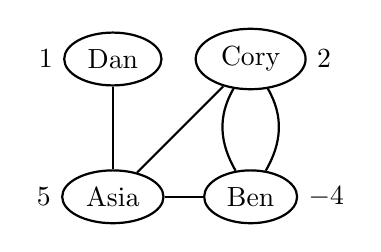
\begin{tikzpicture}[thick,main/.style = {draw, ellipse}]
\begin{scope}[scale=1.75]
    \node[main,label={left:$5$}] (1) at (0,0) {Asia}; 
    \node[main,label={right:$-4$}] (2) at (1,0) {Ben}; 
    \node[main,label={right:$2$}] (3) at (1,1) {Cory};
    \node[main,label={left:$1$}] (4) at (0,1) {Dan};
    \draw[thick] (1) to (2);
    \draw[thick] (2) to [out=60,in=300,looseness=1] (3);
    \draw[thick] (2) to [out=120,in=240,looseness=1] (3);
    \draw[thick] (3) to (1);
    \draw[thick] (1) to (4);
\end{scope}
\end{tikzpicture}
\end{document}
    \caption{A starting distribution in a four-person community.}
    \label{fig 2.1}
\end{figure}

In one move, a person can either fire (lend) money by sending one dollar along each edge, or borrow money by taking one dollar along each edge. Figure \ref{fig 2.2} demonstrates Asia making a firing move and then Ben making a borrowing move. The goal of the game is to redistribute wealth through a sequence of firing and borrowing moves so that everyone has no debt. 

\begin{figure}[ht]
    \centering
    \documentclass{standalone}
\usepackage{tikz}
%------------tikz Setup------------

\tikzstyle{ball} = [circle,shading=ball, ball color=black,
    minimum size=1mm,inner sep=1.3pt]
\tikzstyle{miniball} = [circle,shading=ball, ball color=black,
    minimum size=1mm,inner sep=0.5pt]
\tikzstyle{mminiball} = [circle,shading=ball, ball color=black,
    minimum size=0.6mm,inner sep=0.1pt]
\usetikzlibrary{arrows.meta}
\usetikzlibrary{angles, quotes}
\tikzset{>={Latex[length=2mm,width=1.5mm]}}
\tikzset{->-/.style={decoration={markings, mark=at position #1 with
  {\arrow{>}}},postaction={decorate}}}
\usetikzlibrary{decorations.pathmorphing}
\usetikzlibrary{decorations.pathreplacing}
\usetikzlibrary{arrows.meta,calc}
\usetikzlibrary{bending}
\usetikzlibrary{decorations.markings,shapes.geometric}
\tikzset{->-/.style={decoration={markings, mark=at position #1 with
  {\arrow{>}}},postaction={decorate}}}
\tikzset{-|-/.style={decoration={markings, mark=at position #1 with
  {\arrow{stealth}}},postaction={decorate}}}
\tikzset{movearrow/.style 2 args ={
        decoration={markings,
    mark= at position {#1} with {\arrow{#2}} ,
        },
        postaction={decorate}
    }
}


\begin{document}
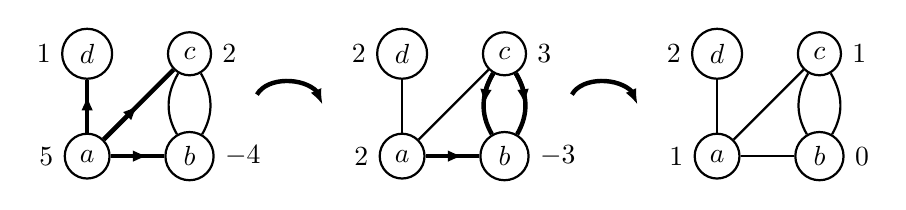
\begin{tikzpicture}[thick,main/.style = {draw, circle}]
\begin{scope}[scale=1.3]
    \node[main,label={left:$5$}] (1) at (0,0) {$a$}; 
    \node[main,label={right:$-4$}] (2) at (1,0) {$b$}; 
    \node[main,label={right:$2$}] (3) at (1,1) {$c$};
    \node[main,label={left:$1$}] (4) at (0,1) {$d$};
    \draw[ultra thick] (1) to (2);
    \draw[thick] (2) to [out=60,in=300,looseness=1] (3);
    \draw[thick] (2) to [out=120,in=240,looseness=1] (3);
    \draw[ultra thick] (3) to (1);
    \draw[ultra thick] (1) to (4);
    \draw[ultra thick,->] (1) to (0, 0.6);
    \draw[ultra thick,->] (1) to (0.6, 0);
    \draw[ultra thick,->] (1) to (0.5, 0.5);
    \node (a) at (1.6, 0.5) {};
    \node (b) at (2.3, 0.4) {};
    \draw[ultra thick,->] (a) to [out=60,in=90] (b);
\end{scope}
\begin{scope}[xshift=4cm,scale=1.3]
    \node[main,label={left:$2$}] (1) at (0,0) {$a$}; 
    \node[main,label={right:$-3$}] (2) at (1,0) {$b$}; 
    \node[main,label={right:$3$}] (3) at (1,1) {$c$};
    \node[main,label={left:$2$}] (4) at (0,1) {$d$};
    \draw[ultra thick] (1) to (2);
    \draw[ultra thick] (2) to [out=60,in=300,looseness=1] (3);
    \draw[ultra thick] (2) to [out=120,in=240,looseness=1] (3);
    \draw[thick] (3) to (1);
    \draw[thick] (1) to (4);
    \draw[ultra thick,->] (1) to (0.6, 0);
    \draw[ultra thick,->] (3) to [out=300,in=90,looseness=1] (1.2,0.5);
    \draw[ultra thick,->] (3) to [out=240,in=90,looseness=1] (0.8,0.5);
    \node (a) at (1.6, 0.5) {};
    \node (b) at (2.3, 0.4) {};
    \draw[ultra thick,->] (a) to [out=60,in=90] (b);
\end{scope}
\begin{scope}[xshift=8cm,scale=1.3]
    \node[main,label={left:$1$}] (1) at (0,0) {$a$}; 
    \node[main,label={right:$0$}] (2) at (1,0) {$b$}; 
    \node[main,label={right:$1$}] (3) at (1,1) {$c$};
    \node[main,label={left:$2$}] (4) at (0,1) {$d$};
    \draw[thick] (1) to (2);
    \draw[thick] (2) to [out=60,in=300,looseness=1] (3);
    \draw[thick] (2) to [out=120,in=240,looseness=1] (3);
    \draw[thick] (3) to (1);
    \draw[thick] (1) to (4);
\end{scope}
\end{tikzpicture}
\end{document}
    \caption{Asia making a firing move, then Ben a borrowing move.}
    \label{fig 2.2}
\end{figure}

We can see from Figure \ref{fig 2.2} that the game is won after just two moves. However, not all games will be as simple. Hence, some questions naturally arise, including
\begin{enumerate}
    \item Are there efficient winning algorithms? (Section \ref{6})
    \label{question 1}
    \item Given a graph, what is the minimum value $x$ such that every distribution with $x$ or more total dollars is winnable? (Section \ref{7})
    \label{question 2}
    \item Are some games more winnable than others? (Section \ref{8}, \ref{9})
    \label{question 3}
\end{enumerate}
We will answer these questions in this paper.





\section{Formal Definitions}
\label{3}

Now that we have introduced the dollar game, we will formally define some related terms which will be referenced throughout the paper. 

\begin{defn}
\label{defn 3.1}
A \textit{divisor} $D$ on graph $G$ is an element of the free abelian group:
\[D\in \text{Div}(G)=\{ \sum_{v\in V}D(v)v:D(v)\in \mathbb{Z} \}.\]
Where $D(v)$ is the amount of dollars on vertex $v$, and $D(v)<0$ indicates debt.
\end{defn}

\begin{defn}
\label{defn 3.2}
The \textit{degree} of a divisor $D\in \text{Div}(G)$ is computed by
\[\text{deg}(D)=\sum_{v\in V}D(v).\]
\end{defn}

For example, the divisor for the initial graph in Figure \ref{fig 2.1} is $D=5a-4b+2c+d$, and $\text{deg}(D)=5-4+2+1=4$. A divisor provides a convenient way to represent a distribution of dollars, and $\text{deg}(D)$ is the total number of dollars in the graph. 

\begin{rem}
We use $\text{deg}_G(v)$ to denote the number of incident edges to a vertex $v\in V$ on graph $G$. Be careful to avoid confusion with $\text{deg}(D)$.
\end{rem}

\begin{defn}
\label{defn 3.3}
Let $D, D'\in \text{Div}(G)$ and $v\in V$. A $\textit{firing move at v}$, denoted $D\xrightarrow{v} D'$, sends a dollar along each of its edges to each adjacent vertex:
\[D'=D-\sum_{vw\in E}(v-w)=D-\text{deg}_G(v)v+\sum_{vw\in E}w.\]
A $\textit{borrowing move at v}$, denoted $D\xrightarrow{-v} D'$, takes a dollar from each adjacent vertex:
\[D'=D+\sum_{vw\in E}(v-w)=D+\text{deg}_G(v)v-\sum_{vw\in E}w.\]
\end{defn}

\begin{rem}
\label{rem 3.1}
Definition \ref{defn 3.3} shows that firing and borrowing moves are made by addition and subtraction on divisors. Thus, the moves are commutative, and can be done in any order or simultaneously and obtain the same result. Furthermore, the degree of a divisor is not changed after firing and borrowing moves.
\end{rem}

\begin{defn}
\label{defn 3.4}
Take a set of vertices $S\subseteq V$. Let $D, D'\in \text{Div}(G)$ and suppose that $D'$ is obtained from $D$ by firing once from each vertex in $S$. This is called a \textit{set-firing} on $D$ by $S$, denoted $D\xrightarrow{S} D'$.
\end{defn}

\begin{exmp}
Below is a set-firing by $\{a,c,d\}$. Vertices $a,c,d$ all fire once. Notice that the result is the same as a borrowing move at $b$, as seen in Figure \ref{fig 2.2}.
\begin{center}
    \documentclass{standalone}
\usepackage{tikz}
%------------tikz Setup------------

\tikzstyle{ball} = [circle,shading=ball, ball color=black,
    minimum size=1mm,inner sep=1.3pt]
\tikzstyle{miniball} = [circle,shading=ball, ball color=black,
    minimum size=1mm,inner sep=0.5pt]
\tikzstyle{mminiball} = [circle,shading=ball, ball color=black,
    minimum size=0.6mm,inner sep=0.1pt]
\usetikzlibrary{arrows.meta}
\usetikzlibrary{angles, quotes}
\tikzset{>={Latex[length=2mm,width=1.5mm]}}
\tikzset{->-/.style={decoration={markings, mark=at position #1 with
  {\arrow{>}}},postaction={decorate}}}
\usetikzlibrary{decorations.pathmorphing}
\usetikzlibrary{decorations.pathreplacing}
\usetikzlibrary{arrows.meta,calc}
\usetikzlibrary{bending}
\usetikzlibrary{decorations.markings,shapes.geometric}
\tikzset{->-/.style={decoration={markings, mark=at position #1 with
  {\arrow{>}}},postaction={decorate}}}
\tikzset{-|-/.style={decoration={markings, mark=at position #1 with
  {\arrow{stealth}}},postaction={decorate}}}
\tikzset{movearrow/.style 2 args ={
        decoration={markings,
    mark= at position {#1} with {\arrow{#2}} ,
        },
        postaction={decorate}
    }
}


\begin{document}
\begin{tikzpicture}
\begin{scope}[scale=2.3]
    \node[ball, label={above:$O$}] (o) at (0,1) {};
    \node[ball] (1) at (-2,0) {};
    \node[ball] (2) at (2,0) {};
    \node[ball] (4) at (-1.5,-0.5) {};
    \node[ball] (3) at (2.5,-0.5) {};
    \draw[dashed] (1) to (2);
    \draw[dashed] (2) to (3);
    \draw[dashed] (3) to (4);
    \draw[dashed] (1) to (4);
    \node[ball] (1a) at (-2,0) {};
    \node[ball] (2a) at (2,-1.5) {};
    \node[ball] (4a) at (-1.5,-0.5) {};
    \node[ball] (3a) at (2.5,-2) {};
    \draw[dashed] (1a) to (2a);
    \draw[dashed] (2a) to (3a);
    \draw[dashed] (3a) to (4a);
    \draw[dashed] (1a) to (4a);
    \node[ball, label={above left:$A$}] (A) at (-0.5,-0.25) {};
    \node[ball, label={above right:$B$}] (B) at (0.5, -0.25) {};
    \node[ball, label={above right:$M$}] (M) at (0, -0.25) {};
    \node[ball, label={left:$A'$}] (A') at (-0.65,-0.65) {};
    \node[ball, label={below right:$B'$}] (B') at (0.93, -1.25) {};
    \node[ball, label={below right:$M'$}] (M') at (0, -0.9) {};
    \draw (A) to (B);
    \draw (A') to (B');
    \draw (o) to (A');
    \draw (o) to (B');
    \draw (o) to (M');
\end{scope}
\end{tikzpicture}
\end{document}
\end{center}
\end{exmp}

\begin{prop}
\label{prop 3.1}
A borrowing move at $v\in V$ is the same as a set-firing by $V\setminus \{v\}$.
\end{prop}
\begin{proof}
A set-firing $D\xrightarrow{V\setminus \{v\}} D'$ is represented as follows.
\begin{align*}
     D'&=D-\sum_{u\in V\setminus \{v\}}\left[\sum_{uw\in E}(u-w)\right]\\
     &=D-\sum_{u\in V}\left[\sum_{uw\in E}(u-w)\right]+\sum_{vw\in E}(v-w)\\
     &=D+\sum_{vw\in E}(v-w).
\end{align*}
\end{proof}

Henceforth, we may use the term \textit{firing moves} when referring to both firing and borrowing moves, since a borrowing move can always be expressed as a set-firing.

\begin{defn}
\label{defn 3.5}
Let $D, D'\in \text{Div}(G)$. If $D'$ can be obtained from $D$ by a sequence of firing moves, we say that $D$ is \textit{linearly equivalent} to $D'$, denoted $D\sim D'$. 
\end{defn}

\begin{prop}
Linear equivalence is an equivalence relation on $\text{Div}(G)$.
\end{prop}
\begin{proof}
The notation $\{v_1\dots v_n\}$ suggests a multiset of vertices.
\begin{enumerate}[(i)]
    \item $D\sim D$ (reflexive). This is clearly true if we make no firing moves.
    \item If $D\sim D'$, then $D'\sim D$ (symmetric). A borrowing move at vertex $v$ undoes a firing move at $v$. Suppose we arrive at $D'$ from $D$ by a sequence of firing moves at $\{v_1,\dots, v_n\}$. We can get back to $D$ from $D'$ by a sequence of borrowing moves at $\{v_1,\dots, v_n\}$.
    \item $D\sim D'$ and $D'\sim D''$, then $D\sim D''$ (transitive). Suppose we arrive at $D'$ from $D$ by a sequence of firing moves at $\{v_1,\dots, v_n\}$ and we arrive at $D'$ from $D''$ by a sequence of firing moves at $\{v_1,\dots, v_m\}$. Then we can arrive at $D''$ from $D$ by a sequence of firing moves at $\{v_1,\dots, v_n,v_1,\dots, v_m\}$.
\end{enumerate}
Hence, linear equivalence is an equivalence relation.
\end{proof}

Lastly, we will define some terms to help us classify winning divisors, in which all vertices are debt-free. For $D, D'\in \text{Div}(G)$, we say $D\geq D'$ if $D(v)\geq D'(v)$ for all $v\in V$, and $D\geq 0$ if $D(v)\geq 0$ for all $v\in V$. 

\begin{defn}
\label{defn 3.6}
A divisor $D\in \text{Div}(G)$ is \textit{effective} if $D\geq 0$.
\end{defn}

\begin{defn}
\label{defn 3.7}
A divisor $D\in \text{Div}(G)$ is \textit{winnable} if $D$ is linearly equivalent to an effective divisor and \textit{unwinnable} otherwise.
\end{defn}





\section{The Laplacian Operator}
\label{4}

In the previous section, we defined \textit{set-firing} as every vertex in $S\subseteq V$ performing a firing move. We can expand on this notion by introducing a function $\sigma: V\rightarrow \mathbb{Z}$. 

\begin{defn}
\label{defn 4.1}
A \textit{firing-script} is a function $\sigma: V\rightarrow \mathbb{Z}$ where $\sigma(v)$ denotes the number firing action on vertex $v$. In other words, if $\sigma(v)>0$ then $v$ fires $\sigma(v)$ times, if $\sigma(v)<0$ then $v$ borrows $\sigma(v)$ times, and if $\sigma(v)=0$ then $v$ does nothing.
\end{defn}

The set of firing-scripts is the set of all integer-valued functions on the vertices of $G$, which forms an abelian group $\mathcal{M}=\text{Hom}(V,\mathbb{Z)}$.

\begin{defn}
\label{defn 4.2}
To map a firing-script to a divisor, we call upon the \textit{discrete Laplacian operator} $\Delta:\mathcal{M}\rightarrow \text{Div}(G)$ with $\Delta(\sigma)=\sum_{v\in V}\Delta_v(\sigma)(v)$ where:
\begin{align*}
    \Delta_v(\sigma)&=\text{deg}(v)\sigma(v)-\sum_{vw\in E}\sigma(w)\\
    &=\sum_{vw\in E}(\sigma(v)-\sigma(w)).
\end{align*}
\end{defn}

By this definition, if we begin with a divisor $D$ on $G$ and implement a firing script $\sigma$, we get $D'=D-\Delta(\sigma)$. All linearly equivalent divisors to $D$ can be reached by implementing a firing script. Let us denote this \textit{script-firing} by $D\xrightarrow{\sigma} D'$. Since the degree of a divisor is preserved under firing moves, we know $\text{deg}(\Delta(\sigma))=0$ for all firing scripts $\sigma$. We can associate a $|V|\times |V|$ matrix $L$ to the Laplacian operator. To do this, first fix an ordering $v_1, v_2,\dots,v_n$ of the vertices of $G$.

\begin{defn}
\label{defn 4.3}
The \textit{Laplacian matrix} $L:\mathbb{Z}^{|V|}\rightarrow \mathbb{Z}^{|V|}$ for a graph $G$ is the linear map defined by
\[L=\text{Diag}(G)-A.\]
where $\text{Diag}(G)$ is the diagonal matrix listing the vertex-degrees of $G$ and $A$ is the \textit{adjacency matrix} of $G$ where $A_{ij}$ is the number of edges between $v_i$ and $v_j$.
\end{defn}
We can compute $L$ entry wise by 
\[L_{ij}=
\begin{cases}
    \text{deg}_G(v_i), & i=j\\
    -(\text{number of edges between }v_i\text{ and }v_j), & i\neq j.
\end{cases}
\]

To perform a firing move at $v_i$, take the column corresponding to $v_i$ and subtract it from a divisor written as a $|V|\times 1$ vector $D$ where $D_{i1}=D(v_i)$. Furthermore, we can write a firing-script as a $|V|\times 1$ vector $x$ where $x_{i1}=\sigma(v_i)$. Then for $D, D'\in \text{Div}(G)$ and $D\xrightarrow{\sigma} D'$, we have the transformation
\[D'=D-Lx.\]

\begin{exmp}
Below is the Laplacian matrix $L$ for the graph from Figure \ref{fig 2.1}.
\begin{center}
    \documentclass{standalone}
\usepackage{tikz}
\usetikzlibrary{matrix,decorations.pathreplacing, calc, positioning,fit}
%------------tikz Setup------------

\tikzstyle{ball} = [circle,shading=ball, ball color=black,
    minimum size=1mm,inner sep=1.3pt]
\tikzstyle{miniball} = [circle,shading=ball, ball color=black,
    minimum size=1mm,inner sep=0.5pt]
\tikzstyle{mminiball} = [circle,shading=ball, ball color=black,
    minimum size=0.6mm,inner sep=0.1pt]
\usetikzlibrary{arrows.meta}
\usetikzlibrary{angles, quotes}
\tikzset{>={Latex[length=2mm,width=1.5mm]}}
\tikzset{->-/.style={decoration={markings, mark=at position #1 with
  {\arrow{>}}},postaction={decorate}}}
\usetikzlibrary{decorations.pathmorphing}
\usetikzlibrary{decorations.pathreplacing}
\usetikzlibrary{arrows.meta,calc}
\usetikzlibrary{bending}
\usetikzlibrary{decorations.markings,shapes.geometric}
\tikzset{->-/.style={decoration={markings, mark=at position #1 with
  {\arrow{>}}},postaction={decorate}}}
\tikzset{-|-/.style={decoration={markings, mark=at position #1 with
  {\arrow{stealth}}},postaction={decorate}}}
\tikzset{movearrow/.style 2 args ={
        decoration={markings,
    mark= at position {#1} with {\arrow{#2}} ,
        },
        postaction={decorate}
    }
}


\begin{document}
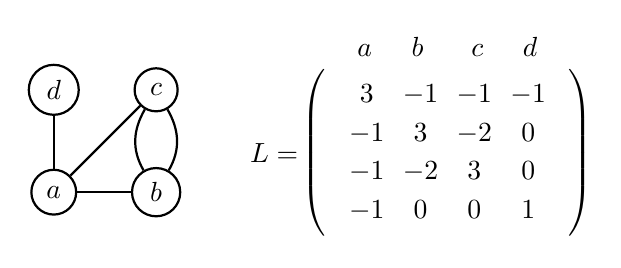
\begin{tikzpicture}[thick,main/.style = {draw, circle}]
\begin{scope}[scale=1.3]
    \node[main] (1) at (0,0) {$a$}; 
    \node[main] (2) at (1,0) {$b$}; 
    \node[main] (3) at (1,1) {$c$};
    \node[main] (4) at (0,1) {$d$};
    \draw[thick] (1) to (2);
    \draw[thick] (2) to [out=60,in=300,looseness=1] (3);
    \draw[thick] (2) to [out=120,in=240,looseness=1] (3);
    \draw[thick] (3) to (1);
    \draw[thick] (1) to (4);
\end{scope}
\begin{scope}[xshift=5cm, yshift=0.5cm]
    \node (a) at (-1.05,1.3) {$a$};
    \node (b) at (-0.38,1.35) {$b$};
    \node (c) at (0.38,1.3) {$c$};
    \node (d) at (1.05,1.35) {$d$};
    \node (l) at (-2.2,0) {$L=$};
    \matrix [matrix of math nodes,left delimiter=(,right delimiter=)](A){ 
    3 & -1 & -1 & -1\\
    -1 & 3 & -2 & 0\\  
    -1 & -2 & 3 & 0\\
    -1 & 0  & 0 & 1\\
    };
\end{scope}
\end{tikzpicture}
\end{document}
\end{center}
If we wanted to represent the moves in Figure \ref{fig 2.2}, namely Asia making a firing move and Ben a borrowing move, we have $D=(5,-4,2,1)^T$ and firing-script $x=(1,-1,0,0)^T$. Then 
\[D'=D-Lx=(5,-4,2,1)^T-(4,-4,1,-1)^T=(1,0,1,2)^T.\]
\end{exmp}

\begin{prop}
\label{prop 4.1}
Consider some firing script $\sigma$. Then $\Delta(\sigma)=0$ if and only if $\sigma$ is constant. 
\end{prop}
\begin{proof}
Suppose $\Delta(\sigma)=0$. Then find vertex $v\in V$ where $\sigma(v)=m$ is maximal. Then we must have 
\[\text{deg}_G(v)\cdot m=\sum_{vw\in E}\sigma(w).\]
We have $\sigma(w)\leq k$, so this only occurs when $\sigma(w)=m$ for all $w$ such that $vw\in E$. Graph $G$ is finite and connected, so $\sigma(v)=m$ for all $v\in V$.
\end{proof}





\section{Q-Reduced Divisors}
\label{5}

To tackle the question of winnability, we will introduce the concept of $q$\textit{-reduced} divisors. Start with a divisor $D\in \text{Div}(G)$. Then follow the steps below to attempt to find an effective divisor $E\sim D$. 

\begin{enumerate}
    \item Choose $q\in V$ and call it the \textit{source} vertex. Denote $\tilde{V}:=V\setminus \{q\}$ as the set of \textit{non-source} vertices.
    \item We want the debt to be concentrated on $q$, so fire from $q$ and share among the vertices of $\tilde{V}$ so that only $q$ is possibly in debt.
    \item Find a nonempty set of vertices $S\subseteq \tilde{V}$ such that if we perform a set-firing on $S$, none of the vertices in $S$ go into debt, called a \textit{legal} set-firing. Then perform a set-firing on $D$ by $S$. Repeat this process until it is impossible to find a legal set-firing, at which point $D$ is $q$\textit{-reduced}.
\end{enumerate}

At the end of this process, if $D(q)\geq 0$, we have found one effective divisor $E$, and the game is winnable! Let us now formally define $q$-reduced divisors.

\begin{defn}
\label{defn 5.1}
Let $q\in V$. Then a divisor $D\in \text{Div}(G)$ is $q$\textit{-reduced} if $D(v)\geq 0$ for all $v\in \tilde{V}:=V\setminus \{q\}$ and for all nonempty $S\subseteq \tilde{V}$, there exists $v\in S$ such that 
\[D(v)<\text{outdeg}_S(v),\]
where $\text{outdeg}_S(v)$ denotes the number of edges $vw$ such that $w\notin S$.
\end{defn}

Before we proceed, we will introduce a different way of viewing graphs, which will be useful in proving upcoming corollaries. 

\begin{defn}
\label{defn 5.2}
A \textit{spanning tree} $T$ is a subset of graph $G$, which has all the vertices covered with minimum possible number of edges. Fix a vertex $v_1=q\in V$ and denote $(T,q)$ as the spanning tree $T$ \textit{rooted} at $q$.
\end{defn}

Let us label the vertices of the spanning tree, $v_1, v_2,\dots,v_n$ where $q=v_1$. This is a \textit{tree ordering} if $i<j$ whenever $v_i$ and $v_j$ are on the same path to $q$ and $v_i$ is closer to $q$ than $v_j$. While spanning trees will not be explored much further in this paper, we will apply the concept of spanning trees to divisors, as we can find a tree ordering on a spanning tree of any divisor. 

\begin{exmp}
The bold edges on the graphs below indicate two possible tree orderings for the graph in Figure \ref{fig 2.1}.
\begin{center}
    \documentclass{standalone}
\usepackage{tikz}
%------------tikz Setup------------

\tikzstyle{ball} = [circle,shading=ball, ball color=black,
    minimum size=1mm,inner sep=1.3pt]
\tikzstyle{miniball} = [circle,shading=ball, ball color=black,
    minimum size=1mm,inner sep=0.5pt]
\tikzstyle{mminiball} = [circle,shading=ball, ball color=black,
    minimum size=0.6mm,inner sep=0.1pt]
\usetikzlibrary{arrows.meta}
\usetikzlibrary{angles, quotes}
\tikzset{>={Latex[length=2mm,width=1.5mm]}}
\tikzset{->-/.style={decoration={markings, mark=at position #1 with
  {\arrow{>}}},postaction={decorate}}}
\usetikzlibrary{decorations.pathmorphing}
\usetikzlibrary{decorations.pathreplacing}
\usetikzlibrary{arrows.meta,calc}
\usetikzlibrary{bending}
\usetikzlibrary{decorations.markings,shapes.geometric}
\tikzset{->-/.style={decoration={markings, mark=at position #1 with
  {\arrow{>}}},postaction={decorate}}}
\tikzset{-|-/.style={decoration={markings, mark=at position #1 with
  {\arrow{stealth}}},postaction={decorate}}}
\tikzset{movearrow/.style 2 args ={
        decoration={markings,
    mark= at position {#1} with {\arrow{#2}} ,
        },
        postaction={decorate}
    }
}


\begin{document}
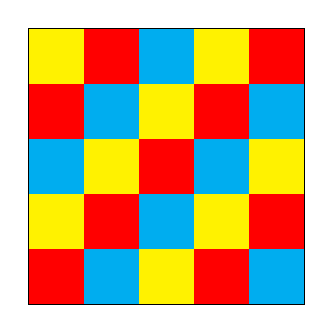
\begin{tikzpicture}[scale=0.7]
    \draw[thick] (0,0) rectangle (5,5);
    \fill[red] (0,0) rectangle (1,1);
    \fill[red] (1,1) rectangle (2,2);
    \fill[red] (2,2) rectangle (3,3);
    \fill[red] (3,3) rectangle (4,4);
    \fill[red] (4,4) rectangle (5,5);
    \fill[red] (3,0) rectangle (4,1);
    \fill[red] (4,1) rectangle (5,2);
    \fill[red] (0,3) rectangle (1,4);
    \fill[red] (1,4) rectangle (2,5);
    \fill[cyan] (1,0) rectangle (2,1);
    \fill[cyan] (2,1) rectangle (3,2);
    \fill[cyan] (3,2) rectangle (4,3);
    \fill[cyan] (4,3) rectangle (5,4);
    \fill[cyan] (0,2) rectangle (1,3);
    \fill[cyan] (1,3) rectangle (2,4);
    \fill[cyan] (2,4) rectangle (3,5);
    \fill[cyan] (4,0) rectangle (5,1);
    \fill[yellow] (0,1) rectangle (1,2);
    \fill[yellow] (1,2) rectangle (2,3);
    \fill[yellow] (2,3) rectangle (3,4);
    \fill[yellow] (3,4) rectangle (4,5);
    \fill[yellow] (2,0) rectangle (3,1);
    \fill[yellow] (3,1) rectangle (4,2);
    \fill[yellow] (4,2) rectangle (5,3);
    \fill[yellow] (0,4) rectangle (1,5);
\end{tikzpicture}
\end{document}
\end{center}
\end{exmp}

\begin{defn}
\label{defn 5.3}
Given $D, D'\in \text{Div}(G)$, first find a spanning tree and then find a tree ordering of the vertices. We say $D'\prec D$ if 
\begin{enumerate}[(i)]
    \item $\text{Deg}(D')<\text{Deg}(D)$
    \item $\text{Deg}(D')=\text{Deg}(D)$ and $D'(v_i)>D(v_i)$ at the smallest index $i$ such that $D'(v_i)\neq D(v_i)$.
\end{enumerate}
\end{defn}

This method of ordering divisors essentially tells you that $D'\prec D$ if on $D'$, more money is closer to the source vertex, $q$. We will see in the following lemma one key property of the tree ordering rooted at $q$, which will be used to prove Theorem \ref{thm 5.1}.

\begin{lem}
\label{lem 5.1}
Let $D, D'\in \textup{Div}(G)$ and $q\in V$. Let $D'$ be the result of firing a nonempty set $S\subseteq \tilde{V}:=V\setminus \{q\}$ on $D$. Then $D'\prec D$.
\end{lem}
\begin{proof}
Consider a tree ordering of the spanning tree $(T, q)$ on $D$ where $q=v_1$. Let $v_j$ be the vertex with the smallest index such that $v_j$ is incident to an element of $S$. Upon firing $S$, the degree of $D$ stays the same and $D(v_i)=D'(v_i)$ for $j=2,\dots,j-1$, but $D(v_j)<D'(v_j)$. Thus, $D'\prec D$ by definition. 
\end{proof}

\begin{thm}
\label{thm 5.1}
Let $D\in \textup{Div}(G)$, and fix $q\in V$. Then there exists a unique $q$-reduced  divisor $D_q \sim D$.
\end{thm}
\begin{proof}
Consider a tree ordering of the spanning tree $(T, q)$ on $D$ where $q=v_1$. We can cancel all the debt on $v_n, v_{n-1},\dots,v_2$, in that order, by lending at their respective neighbors.

We will now show existence. If $D$ is already $q$-reduced, we are done. Otherwise, perform a legal set-firing on a nonempty set $S\subseteq \tilde{V}:=V\setminus \{q\}$ to obtain $D_1$. By Lemma \ref{lem 5.1}, $D\succ D_1$. We can always repeat this process to get $D \succ D_1 \succ D_2 \dots$. Since the set $\tilde{V}$ is finite and we only perform legal set firings, meaning $D(v)\geq 0$ for all $v\in \tilde{V}$, we always reach a divisor $D_i$ on which we can no longer find a legal set-firing, at which point $D$ is $q$-reduced.

We will then show uniqueness by contradiction. Assume that $D_q$ and $D_q'$ are two $q-$reduced divisors linearly equivalent to $D$ and each other, i.e. $D\sim D_q\sim D_q'$. Then $D_q'=D_q-\Delta(\sigma)$ for some firing script $\sigma$. Let $S$ be the set of vertices on which $\sigma$ is maximized. By Proposition \ref{prop 4.1}, $\sigma$ cannot be constant, so $S\neq V$. Furthermore, if $q\in S$, we swap $D_q$ with $D_q'$ so that $\sigma$ becomes $-\sigma$, so $q\notin S$. For each $v\in S$ and $w\notin S$, we have
\[0\leq D_q'(v)=D_q(v)-\sum_{vw\in E}(\sigma(v)-\sigma(w))\leq D_q(v)-\text{outdeg}_S(v).\]
Then $D_q(v)\geq \text{outdeg}_S(v)$, so we can legally fire $S$, and $D_q$ is not $q$-reduced.
\end{proof}

\begin{cor}
\label{cor 5.1}
Let $D, D' \in \textup{Div}(G)$ be divisors and let $D_q, D_q'$ be their $q$-reduced  equivalent divisors respectively. Then $D\sim D'$ if and only if $D_q\sim D_q'$.
\end{cor}
\begin{proof}
This follows from the uniqueness of $q$-reduced divisors.
\end{proof}

\begin{cor}
\label{cor 5.2}
Let $D \in \textup{Div}(G)$ be a divisor and $D_q$ its $q$-reduced equivalent
divisor, then $D$ is winnable if and only if $D_q(q)\geq 0$.
\end{cor}
\begin{proof}
To prove the forward direction, we must show that if $D$ is winnable, then $D_q(q)\geq 0$. First note that $D\sim E$, an effective divisor. Then $D\sim E_q$, the $q$-reduced effective divisor. We know that $D_q=E_q$ by uniqueness. Furthermore, when we $q$-reduce $E$ to $E_q$, we never fire from $q$ since all vertices are already non-negative. Thus, $D_q(q)\geq 0$. The backward direction is trivial.
\end{proof}





\section{Dhar's Burning Algorithm}
\label{6}

Based on the implications of Corollaries \ref{cor 5.1} and \ref{cor 5.2}, we now see the importance of determining the $q$-reduced  divisor. Before we introduce an algorithm that does just this, let us first define some useful terminology that will be quite intuitive in light of our discussion of divisors.

\begin{defn}
\label{defn 6.1}
Fix a vertex $q\in V$ and define $\tilde{V}:=V\setminus \{q\}$. Then a \textit{configuration} on $G$ is an element of the subgroup
\[c\in \text{Config}(G,q)=\{\sum_{v\in \tilde{V}}c(v)v:c(v)\in \mathbb{Z}\}\subset \text{Div}(G).\]
\end{defn}

Put simply, a configuration $c$ is a divisor that excludes some vertex $q$. We may still fire from and borrow at $q$ as with divisors, but vertex $q$ does not appear in the expression for $c$. Notation is similar to that of divisors. The \textit{degree} of a configuration $c$ is computed by $\text{deg}(c)=\sum_{v\in \tilde{V}}c(v)$. For $c, c'\in \text{Config}(G,q)$, we say $c\geq c'$ if $c(v)\geq c'(v)$ for all $c\in V$ and $c\geq 0$ if $c(v)\geq 0$ for all $c\in V$. Finally, $c$ and $c'$ are \textit{linearly equivalent}, denoted $c\sim c'$ if they can be obtained from one another by firing and borrowing moves. Note that unlike with divisors, two linearly equivalent divisors do not necessarily have the same degree. A set-firing on the vertices in $S\subseteq \tilde{V}$ on $c\in \text{Config}(G)$, denoted $c\xrightarrow{S} c'$ is \textit{legal} if for all $v\in S$, $c'(v)\geq 0$.

\begin{defn}
\label{defn 6.3}
A configuration $c\in \text{Config}(G,q)$ is \textit{superstable} if $c\geq 0$ and no set firing is legal, i.e. for all nonempty $S\subseteq \tilde{V}$, there exists some $v\in S$ such that $c(v)<\text{outdeg}_S(v)$ so that firing on $v$ yields $c'(v)<0$.
\end{defn}

\begin{exmp}
A superstable configuration on the graph below is $c=v_2+2v_3$.
\begin{center}
    \documentclass{standalone}
\usepackage{tikz}
%------------tikz Setup------------

\tikzstyle{ball} = [circle,shading=ball, ball color=black,
    minimum size=1mm,inner sep=1.3pt]
\tikzstyle{miniball} = [circle,shading=ball, ball color=black,
    minimum size=1mm,inner sep=0.5pt]
\tikzstyle{mminiball} = [circle,shading=ball, ball color=black,
    minimum size=0.6mm,inner sep=0.1pt]
\usetikzlibrary{arrows.meta}
\usetikzlibrary{angles, quotes}
\tikzset{>={Latex[length=2mm,width=1.5mm]}}
\tikzset{->-/.style={decoration={markings, mark=at position #1 with
  {\arrow{>}}},postaction={decorate}}}
\usetikzlibrary{decorations.pathmorphing}
\usetikzlibrary{decorations.pathreplacing}
\usetikzlibrary{arrows.meta,calc}
\usetikzlibrary{bending}
\usetikzlibrary{decorations.markings,shapes.geometric}
\tikzset{->-/.style={decoration={markings, mark=at position #1 with
  {\arrow{>}}},postaction={decorate}}}
\tikzset{-|-/.style={decoration={markings, mark=at position #1 with
  {\arrow{stealth}}},postaction={decorate}}}
\tikzset{movearrow/.style 2 args ={
        decoration={markings,
    mark= at position {#1} with {\arrow{#2}} ,
        },
        postaction={decorate}
    }
}


\begin{document}
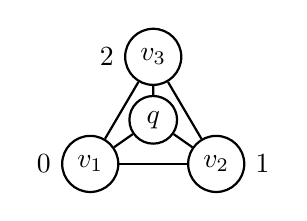
\begin{tikzpicture}[thick,main/.style = {draw, circle}]
\begin{scope}[scale=0.8]
    \node[main,label={left:$0$}] (1) at (0,0) {$v_1$}; 
    \node[main,label={right:$1$}] (2) at (2,0) {$v_2$}; 
    \node[main,label={left:$2$}] (3) at (1,1.7) {$v_3$};
    \node[main] (4) at (1,0.7) {$q$};
    \draw[thick] (1) to (2);
    \draw[thick] (2) to (3);
    \draw[thick] (3) to (1);
    \draw[thick] (1) to (4);
    \draw[thick] (2) to (4);
    \draw[thick] (3) to (4);
\end{scope}
\end{tikzpicture}
\end{document}
\end{center}
\end{exmp}

\begin{rem}
\label{rem 6.1}
Every divisor $D$ can be expressed as $c+kq$, where $c\in \text{Config}(G,q)$ and $k\in \mathbb{Z}$. Thus, $D$ is $q$-reduced if and only if $c$ is superstable. 
\end{rem}

From here we can now explain \textit{Dhar's burning algorithm}, which quickly finds a nonempty legal set-firing for $c$, if one exists at all. This algorithm effectively saves us from having to iterate through all $2^{|\tilde{V}|}-1$ nonempty subsets to determine whether a configuration is superstable.

\RestyleAlgo{ruled}
\SetKwComment{Comment}{/* }{ */}
\begin{algorithm}
\caption{Dhar's burning algorithm}\label{alg 6.1}
\KwData{$c\in\text{Config}(G,q), c\geq 0$}
\KwResult{a legal set firing $S\subset \tilde{V}$, or $S=\emptyset$ iff $c$ is superstable}
$S \gets \tilde{V}$\;
\While{$S \neq \emptyset$}{
  \eIf{$c(v)<\textup{outdeg}_S(v)$ $\textup{for some}$ $v\in S$}{
    $S=S\setminus\{v\}$\Comment*{$c$ is not superstable}
  }{\Return S\;}
}
\Return S\;
\end{algorithm}

We can think of Dhar's algorithm in terms of fires and firemen. Start with $c\in \text{Config}(G,q)$, with $c\geq 0$, since this is the first requirement for being superstable. Imagine there are $c(v)$ firemen on each vertex $v\in \tilde{V}$. First set fire to vertex $q$, which will then set fire to its incident edges. A fireman can control at most one burning edge, so a vertex is protected until there are more incoming fires than firemen. When a vertex ignites, the fire continues to spread along its incident edges. When the algorithm terminates, the set of unburnt vertices can be fired legally. By definition, the configuration $c$ is superstable if the set is empty. We will now prove the validity of Dhar's burning algorithm.

\begin{proof}
Refer to Algorithm \ref{alg 6.1}. When $S$ is returned, it has $c(v)\geq \text{outdeg}_S(v)$ for all $v\in S$, so it is a legal firing set. We must now show 
\[S=\emptyset \Longleftrightarrow c \text{ is superstable}.\]
To prove the forward direction, suppose $S=\emptyset$ upon termination. Let $T\subseteq\tilde{V}$ be any nonempty subset. At the start of the algorithm, $T\subseteq\tilde{V}=S$. At termination, $S=\emptyset$ and $T$ is nonempty, so there exists a vertex $v$ that is the first vertex in $T$ to be removed from $S$. Before $v$ is removed, we know that $T$ is still a subset of $S$ and $c(v)<\textup{outdeg}_S(v)$. Notice that if $T\subseteq S$, then $\textup{outdeg}_S(v)\leq \textup{outdeg}_T(v)$. Hence, $c(v)<\textup{outdeg}_T(v)$. Therefore, $T$ is not a legal firing set for $c$, so $c$ is superstable. The backward direction follows by Definition \ref{defn 6.3}.
\end{proof}

\begin{exmp}
We can run Dhar's burning algorithm on $c=2v_3+v_4$. 
\begin{center}
    \documentclass{standalone}
\usepackage{tikz}
%------------tikz Setup------------

\tikzstyle{ball} = [circle,shading=ball, ball color=black,
    minimum size=1mm,inner sep=1.3pt]
\tikzstyle{miniball} = [circle,shading=ball, ball color=black,
    minimum size=1mm,inner sep=0.5pt]
\tikzstyle{mminiball} = [circle,shading=ball, ball color=black,
    minimum size=0.6mm,inner sep=0.1pt]
\usetikzlibrary{arrows.meta}
\usetikzlibrary{angles, quotes}
\tikzset{>={Latex[length=2mm,width=1.5mm]}}
\tikzset{->-/.style={decoration={markings, mark=at position #1 with
  {\arrow{>}}},postaction={decorate}}}
\usetikzlibrary{decorations.pathmorphing}
\usetikzlibrary{decorations.pathreplacing}
\usetikzlibrary{arrows.meta,calc}
\usetikzlibrary{bending}
\usetikzlibrary{decorations.markings,shapes.geometric}
\tikzset{->-/.style={decoration={markings, mark=at position #1 with
  {\arrow{>}}},postaction={decorate}}}
\tikzset{-|-/.style={decoration={markings, mark=at position #1 with
  {\arrow{stealth}}},postaction={decorate}}}
\tikzset{movearrow/.style 2 args ={
        decoration={markings,
    mark= at position {#1} with {\arrow{#2}} ,
        },
        postaction={decorate}
    }
}


\begin{document}
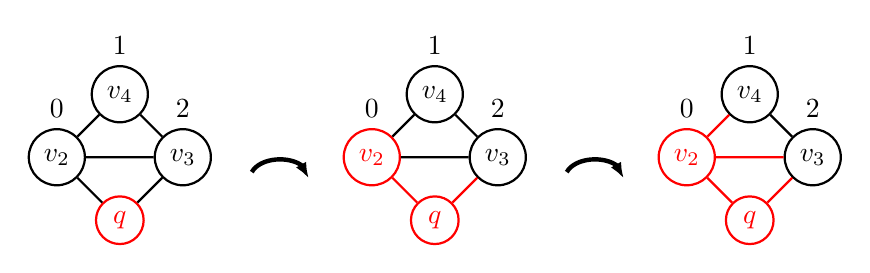
\begin{tikzpicture}[thick,main/.style = {draw, circle}]
\begin{scope}[scale=0.8]
    \node[main,red] (1) at (0,0) {$q$}; 
    \node[main,label={above:$0$}] (2) at (-1,1) {$v_2$};
    \node[main,label={above:$2$}] (3) at (1,1) {$v_3$};
    \node[main,label={above:$1$}] (4) at (0,2) {$v_4$};
    \draw[thick] (1) to (2);
    \draw[thick] (1) to (3);
    \draw[thick] (2) to (4);
    \draw[thick] (3) to (4);
    \draw[thick] (2) to (3);
    \node (a) at (2, 0.6) {};
    \node (b) at (3, 0.5) {};
    \draw[ultra thick,->] (a) to [out=60,in=90] (b);
\end{scope}
\begin{scope}[xshift=4cm,scale=0.8]
    \node[main,red] (1) at (0,0) {$q$}; 
    \node[main,red,label={above:$0$}] (2) at (-1,1) {$v_2$};
    \node[main,label={above:$2$}] (3) at (1,1) {$v_3$};
    \node[main,label={above:$1$}] (4) at (0,2) {$v_4$};
    \draw[thick,red] (1) to (2);
    \draw[thick,red] (1) to (3);
    \draw[thick] (2) to (4);
    \draw[thick] (3) to (4);
    \draw[thick] (2) to (3);
    \node (a) at (2, 0.6) {};
    \node (b) at (3, 0.5) {};
    \draw[ultra thick,->] (a) to [out=60,in=90] (b);
\end{scope}
\begin{scope}[xshift=8cm,scale=0.8]
    \node[main,red] (1) at (0,0) {$q$}; 
    \node[main,red,label={above:$0$}] (2) at (-1,1) {$v_2$};
    \node[main,label={above:$2$}] (3) at (1,1) {$v_3$};
    \node[main,label={above:$1$}] (4) at (0,2) {$v_4$};
    \draw[thick,red] (1) to (2);
    \draw[thick,red] (1) to (3);
    \draw[thick,red] (2) to (4);
    \draw[thick] (3) to (4);
    \draw[thick,red] (2) to (3);
\end{scope}
\end{tikzpicture}
\end{document}
\end{center}
In the end, we can legally fire $S=\{v_3,v_4\}\in \tilde{V}$. Any divisor of the form $D=c+kq$ on this graph, therefore, is NOT $q$-reduced.
\end{exmp}

We have now found an effiecient winning algorithm, answering Question \ref{question 1}! Let us add to our instructions from the beginning of Section \ref{5}. 

\begin{enumerate}
    \item Choose $q\in V$ and call it the \textit{source} vertex. Denote $\tilde{V}:=V\setminus \{q\}$ as the set of \textit{non-source} vertices.
    \item We want the debt to be concentrated on $q$, so fire from $q$ and share among the vertices of $\tilde{V}$ so that only $q$ is in debt.
    \item Iterate through Algorithm \ref{alg 6.1} on $c\in \text{Config}(G,q)$.
    \item When we arrive upon a superstable configuration, $D$ has been $q$-reduced to $D_q$. We can calculate the number of chips are on $q$ using the fact that $\text{deg}(D)$ is constant:
    \[D_q(q)=\text{deg}(D)-\text{deg}(c).\]
    \item By Corollary \ref{cor 5.2}, if $D_q(q)\geq 0$, we have won the dollar game! Otherwise, the game is unwinnable.
\end{enumerate}





\section{Orientations}
\label{7}

Our goal in this section is to find a bijection between \textit{acyclic orientations with unique source} $q$ and \textit{maximal unwinnable }$q$\textit{-reduced divisors}, which will be needed in the proof of Riemann-Roch for graphs (Theorem \ref{thm 8.1}).

\begin{defn}
A graph \textit{orientation} $\mathcal{O}$ chooses a direction for each edge.
\end{defn}

For each edge $vw\in E$, denote $e^-=v$ to be the \textit{tail} and $e^+=w$ to be the \textit{head}, so that $e$ is an arrow from $v$ to $w$. The \textit{reverse orientation} of $\mathcal{O}$, denoted $\overline{\mathcal{O}}$, reverses the head and tail of each edge.

\begin{defn}
\label{defn 7.1}
For each vertex $v\in V$ and an orientation $\mathcal{O}$, the \textit{indegree} is the number of edges pointed towards $v$ and the \textit{outdegree} is the number of edges pointed away from $v$. More formally,
\begin{align*}
    \text{indeg}_{\mathcal{O}}(v)&=|\{e\in \mathcal{O}:e^+=v\}|\\
    \text{outdeg}_{\mathcal{O}}(v)&=|\{e\in \mathcal{O}:e^-=v\}|.
\end{align*}
\end{defn}

A vertex $v\in V$ is a \textit{source} if $\text{indeg}_{\mathcal{O}}(v)=0$ and a \textit{sink} if $\text{outdeg}_{\mathcal{O}}(v)=0$. Be careful not to confuse $\text{indeg}_{\mathcal{O}}(v)$ with $\text{outdeg}_S(v)$, which denotes the number of edges $vw$ such that $w\notin S$ for $S\subseteq \tilde{V}$. We can use indegrees and outdegrees of the vertices to write divisors.

\begin{defn}
\label{defn 7.2}
The divisor corresponding to an orientation $\mathcal{O}$ of $G$ is 
\[\textbf{D}(\mathcal{O})=\sum_{v\in V}(\text{indeg}_{\mathcal{O}}(v)-1)v.\]
The configuration with source $q\in V$ corresponding to $\mathcal{O}$ is
\[\textbf{c}(\mathcal{O})=\sum_{v\in \tilde{V}}(\text{indeg}_{\mathcal{O}}(v)-1)v.\]
\end{defn}

\begin{defn}
\label{defn 7.3}
The \textit{canonical divisor} of a graph $G$ is defined to be 
\[K:=\mathbf{D}(\mathcal{O})+\mathbf{D}(\overline{\mathcal{O}})\]
\end{defn}

Note that the canonical divisor is independent of the choice of orientation $\mathcal{O}$, since for every $v\in V$, 
\[K(v)=(\text{indeg}_{\mathcal{O}}(v)-1)+(\text{outdeg}_{\mathcal{O}}(v)-1)=\text{deg}_{G}(v)-2.\]
Equivalently, the canonical divisor is defined
\[K:=\sum_{v\in V} (\text{deg}_G(v)-2)v.\]
We will revisit the canonical divisor in Section \ref{8}.

For an orientation $\mathcal{O}$, a \textit{directed path} is a path where each vertex is the head of the previous edge and the tail of the next one, and each vertex is unique except for possibly the first and the last. A \textit{directed cycle} is a directed path where the first and last vertices coincide.

\begin{exmp}
Three different orientations are shown below. Orientation $\mathcal{O}_c$ is the reverse orientation of $\mathcal{O}_a$, denoted $\overline{\mathcal{O}}_a$. 
\begin{center}
    \documentclass{standalone}
\usepackage{tikz}
%------------tikz Setup------------

\tikzstyle{ball} = [circle,shading=ball, ball color=black,
    minimum size=1mm,inner sep=1.3pt]
\tikzstyle{miniball} = [circle,shading=ball, ball color=black,
    minimum size=1mm,inner sep=0.5pt]
\tikzstyle{mminiball} = [circle,shading=ball, ball color=black,
    minimum size=0.6mm,inner sep=0.1pt]
\usetikzlibrary{arrows.meta}
\usetikzlibrary{angles, quotes}
\tikzset{>={Latex[length=2mm,width=1.5mm]}}
\tikzset{->-/.style={decoration={markings, mark=at position #1 with
  {\arrow{>}}},postaction={decorate}}}
\usetikzlibrary{decorations.pathmorphing}
\usetikzlibrary{decorations.pathreplacing}
\usetikzlibrary{arrows.meta,calc}
\usetikzlibrary{bending}
\usetikzlibrary{decorations.markings,shapes.geometric}
\tikzset{->-/.style={decoration={markings, mark=at position #1 with
  {\arrow{>}}},postaction={decorate}}}
\tikzset{-|-/.style={decoration={markings, mark=at position #1 with
  {\arrow{stealth}}},postaction={decorate}}}
\tikzset{movearrow/.style 2 args ={
        decoration={markings,
    mark= at position {#1} with {\arrow{#2}} ,
        },
        postaction={decorate}
    }
}


\begin{document}
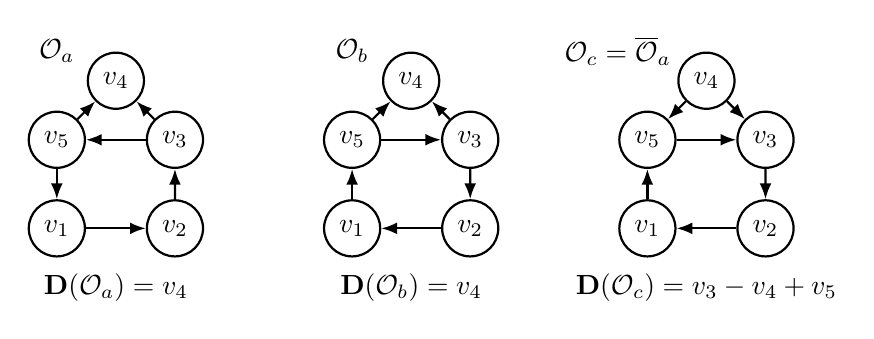
\begin{tikzpicture}[thick,main/.style = {draw, circle}]
\begin{scope}[scale=0.75]
    \node (o) at (0,3) {$\mathcal{O}_a$};
    \node (l) at (1,-1) {$\textbf{D}(\mathcal{O}_a)=v_4$};
    \node[main] (1) at (0,0) {$v_1$}; 
    \node[main] (2) at (2,0) {$v_2$}; 
    \node[main] (3) at (2,1.5) {$v_3$};
    \node[main] (4) at (1,2.5) {$v_4$};
    \node[main] (5) at (0,1.5) {$v_5$};
    \draw[thick,->] (1) to (2);
    \draw[thick,->] (2) to (3);
    \draw[thick,->] (3) to (5);
    \draw[thick,->] (5) to (1);
    \draw[thick,->] (3) to (4);
    \draw[thick,->] (5) to (4);
\end{scope}
\begin{scope}[scale=0.75,xshift=5cm]
    \node (o) at (0,3) {$\mathcal{O}_b$};
    \node (l) at (1,-1) {$\textbf{D}(\mathcal{O}_b)=v_4$};
    \node[main] (1) at (0,0) {$v_1$}; 
    \node[main] (2) at (2,0) {$v_2$}; 
    \node[main] (3) at (2,1.5) {$v_3$};
    \node[main] (4) at (1,2.5) {$v_4$};
    \node[main] (5) at (0,1.5) {$v_5$};
    \draw[thick,->] (2) to (1);
    \draw[thick,->] (3) to (2);
    \draw[thick,->] (5) to (3);
    \draw[thick,->] (1) to (5);
    \draw[thick,->] (3) to (4);
    \draw[thick,->] (5) to (4);
\end{scope}
\begin{scope}[scale=0.75,xshift=10cm]
    \node (o) at (-0.5,3) {$\mathcal{O}_c=\overline{\mathcal{O}}_a$};
    \node (l) at (1,-1) {$\textbf{D}(\mathcal{O}_c)=v_3-v_4+v_5$};
    \node[main] (1) at (0,0) {$v_1$}; 
    \node[main] (2) at (2,0) {$v_2$}; 
    \node[main] (3) at (2,1.5) {$v_3$};
    \node[main] (4) at (1,2.5) {$v_4$};
    \node[main] (5) at (0,1.5) {$v_5$};
    \draw[thick,->] (2) to (1);
    \draw[thick,->] (3) to (2);
    \draw[thick,->] (5) to (3);
    \draw[thick,->] (1) to (5);
    \draw[thick,->] (4) to (3);
    \draw[thick,->] (4) to (5);
\end{scope}
\end{tikzpicture}
\end{document}
\end{center}
Notice that there are two different orientations $\mathcal{O}_a$ and $\mathcal{O}_b$ with coinciding divisors. Thus, the map from orientations to divisors is not injective. This is a problem if we are to find any sort of bijection. The orientation $\mathcal{O}_b$ results from reversing the directed cycle $[v_1,v_2,v_3,v_5,v_1]$ of $\mathcal{O}_a$. When a cycle is reversed, $\text{indeg}_{\mathcal{O}}(v)$ and $\text{outdeg}_{\mathcal{O}}(v)$ for each vertex $v$ in the cycle does not change. Hence why $\mathcal{O}_a$ and $\mathcal{O}_b$ have the same divisor. To fix this problem, we introduce \textit{acyclic} orientations.
\end{exmp}

\begin{defn}
\label{defn 7.4}
An orientation $\mathcal{O}$ is \textit{acyclic} if it contains no directed cycles.
\end{defn}

\begin{figure}[ht]
    \centering
    \documentclass{standalone}
\usepackage{tikz}
%------------tikz Setup------------

\tikzstyle{ball} = [circle,shading=ball, ball color=black,
    minimum size=1mm,inner sep=1.3pt]
\tikzstyle{miniball} = [circle,shading=ball, ball color=black,
    minimum size=1mm,inner sep=0.5pt]
\tikzstyle{mminiball} = [circle,shading=ball, ball color=black,
    minimum size=0.6mm,inner sep=0.1pt]
\usetikzlibrary{arrows.meta}
\usetikzlibrary{angles, quotes}
\tikzset{>={Latex[length=2mm,width=1.5mm]}}
\tikzset{->-/.style={decoration={markings, mark=at position #1 with
  {\arrow{>}}},postaction={decorate}}}
\usetikzlibrary{decorations.pathmorphing}
\usetikzlibrary{decorations.pathreplacing}
\usetikzlibrary{arrows.meta,calc}
\usetikzlibrary{bending}
\usetikzlibrary{decorations.markings,shapes.geometric}
\tikzset{->-/.style={decoration={markings, mark=at position #1 with
  {\arrow{>}}},postaction={decorate}}}
\tikzset{-|-/.style={decoration={markings, mark=at position #1 with
  {\arrow{stealth}}},postaction={decorate}}}
\tikzset{movearrow/.style 2 args ={
        decoration={markings,
    mark= at position {#1} with {\arrow{#2}} ,
        },
        postaction={decorate}
    }
}


\begin{document}
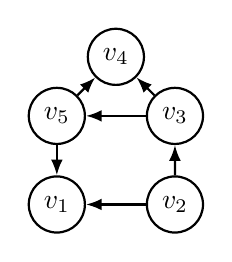
\begin{tikzpicture}[thick,main/.style = {draw, circle}]
\begin{scope}[scale=0.75]
    \node[main] (1) at (0,0) {$v_1$}; 
    \node[main] (2) at (2,0) {$v_2$}; 
    \node[main] (3) at (2,1.5) {$v_3$};
    \node[main] (4) at (1,2.5) {$v_4$};
    \node[main] (5) at (0,1.5) {$v_5$};
    \draw[thick,->] (2) to (1);
    \draw[thick,->] (2) to (3);
    \draw[thick,->] (3) to (5);
    \draw[thick,->] (5) to (1);
    \draw[thick,->] (3) to (4);
    \draw[thick,->] (5) to (4);
\end{scope}
\end{tikzpicture}
\end{document}
    \caption{An acyclic orientation with unique source $v_2$}
    \label{fig 7.2}
\end{figure}

\begin{prop}
\label{prop 7.1}
Every acyclic orientation has at least one source.
\end{prop}
\begin{proof}
For the sake of contradiction, suppose $\mathcal{O}$ has no sources, then $\overline{\mathcal{O}}$ has no sinks. This means as we move along the edges of $\overline{\mathcal{O}}$, at every vertex, there will always be an edge to exit out of. We can continue moving indefinitely, and since the graph is finite, we will eventually visit a vertex twice. Thus, we have found a cycle in $\overline{\mathcal{O}}$, so $\mathcal{O}$ also has a cycle, a contradiction.
\end{proof}

\begin{lem}
\label{lem 7.1}
The map $\{\text{acyclic orientations on }G\} \rightarrow \textup{Config}(G,q)$ given by $\mathcal{O}\mapsto \textbf{c}({\mathcal{O}})$ is injective.
\end{lem}
\begin{proof}
We must show that if $\mathcal{O}$ and $\mathcal{O'}$ are acyclic orientations such that $\textbf{c}(\mathcal{O})=\textbf{c}(\mathcal{O'})$, then $\mathcal{O}=\mathcal{O'}$. Since $q$ is the source, $\text{indeg}_{\mathcal{O}}(q)=\text{indeg}_{\mathcal{O'}}(q)$. So our condition becomes $\text{indeg}_{\mathcal{O}}(v)=\text{indeg}_{\mathcal{O'}}(v)$ for all $v\in V$. By Proposition \ref{prop 7.1}, we can select the nonempty set $V_1\subset V$ of source vertices, namely, vertices with $\text{indeg}_{\mathcal{O}}(v)=0$. Removing source vertices and their incident edges preserves the acyclic property, so we do this for $v\in V_1$ to obtain acyclic $\mathcal{O}_1$ on a subgraph $G_1$ of $G$. Continue this process by selecting the nonempty set $V_2\subset V$, and so forth. When finished, we will have partitioned $V$ into $(V_1,V_2\dots)$. Notice that $\text{indeg}_{\mathcal{O}}(v)$ uniquely determines the partition, which uniquely determines $\mathcal{O}$.
\end{proof}

We can now reinterpret Dhar's burning algorithm with orientations in mind. Start with a superstable configuration $c$ (this will ensure that all edges are burned) and place $c(v)$ firefighters on each vertex $v\in \tilde{V}$. Start a fire on the source vertex $q$ and proceed with Dhar's burning algorithm. The difference now is that whenever a vertex burns, make all the edges that burned the vertex point towards it. An example of this is illustrated in Figure \ref{fig 7.3}.

\begin{figure}[ht]
    \centering
    \documentclass{standalone}
\usepackage{tikz}
%------------tikz Setup------------

\tikzstyle{ball} = [circle,shading=ball, ball color=black,
    minimum size=1mm,inner sep=1.3pt]
\tikzstyle{miniball} = [circle,shading=ball, ball color=black,
    minimum size=1mm,inner sep=0.5pt]
\tikzstyle{mminiball} = [circle,shading=ball, ball color=black,
    minimum size=0.6mm,inner sep=0.1pt]
\usetikzlibrary{arrows.meta}
\usetikzlibrary{angles, quotes}
\tikzset{>={Latex[length=2mm,width=1.5mm]}}
\tikzset{->-/.style={decoration={markings, mark=at position #1 with
  {\arrow{>}}},postaction={decorate}}}
\usetikzlibrary{decorations.pathmorphing}
\usetikzlibrary{decorations.pathreplacing}
\usetikzlibrary{arrows.meta,calc}
\usetikzlibrary{bending}
\usetikzlibrary{decorations.markings,shapes.geometric}
\tikzset{->-/.style={decoration={markings, mark=at position #1 with
  {\arrow{>}}},postaction={decorate}}}
\tikzset{-|-/.style={decoration={markings, mark=at position #1 with
  {\arrow{stealth}}},postaction={decorate}}}
\tikzset{movearrow/.style 2 args ={
        decoration={markings,
    mark= at position {#1} with {\arrow{#2}} ,
        },
        postaction={decorate}
    }
}


\begin{document}
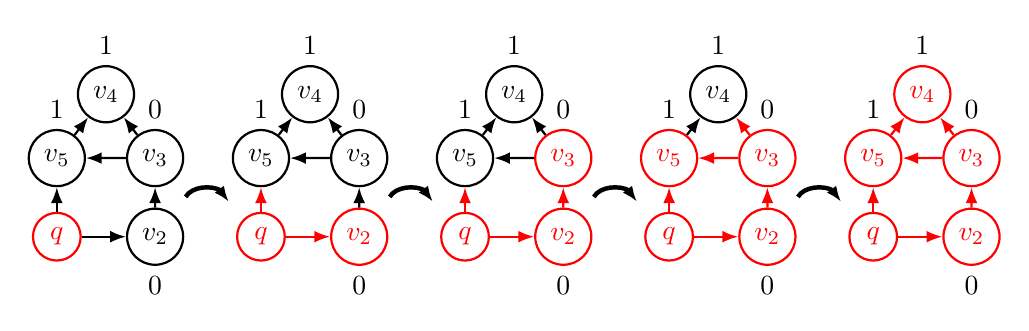
\begin{tikzpicture}[thick,main/.style = {draw, circle},scale=0.96]
\begin{scope}[scale=0.65]
    \node[main,red] (1) at (0,0) {$q$}; 
    \node[main,label={below:$0$}] (2) at (2,0) {$v_2$}; 
    \node[main,label={above:$0$}] (3) at (2,1.6) {$v_3$};
    \node[main,label={above:$1$}] (4) at (1,2.9) {$v_4$};
    \node[main,label={above:$1$}] (5) at (0,1.6) {$v_5$};
    \draw[thick,->] (1) to (2);
    \draw[thick,->] (1) to (5);
    \draw[thick,->] (2) to (3);
    \draw[thick,->] (3) to (5);
    \draw[thick,->] (3) to (4);
    \draw[thick,->] (5) to (4);
    \node (a) at (2.5, 0.6) {};
    \node (b) at (3.5, 0.5) {};
    \draw[ultra thick,->] (a) to [out=60,in=90] (b);
\end{scope}
\begin{scope}[xshift=2.7cm,scale=0.65]
    \node[main,red] (1) at (0,0) {$q$}; 
    \node[main,red,label={below:$0$}] (2) at (2,0) {$v_2$}; 
    \node[main,label={above:$0$}] (3) at (2,1.6) {$v_3$};
    \node[main,label={above:$1$}] (4) at (1,2.9) {$v_4$};
    \node[main,label={above:$1$}] (5) at (0,1.6) {$v_5$};
    \draw[thick,->,red] (1) to (2);
    \draw[thick,->,red] (1) to (5);
    \draw[thick,->] (2) to (3);
    \draw[thick,->] (3) to (5);
    \draw[thick,->] (3) to (4);
    \draw[thick,->] (5) to (4);
    \node (a) at (2.5, 0.6) {};
    \node (b) at (3.5, 0.5) {};
    \draw[ultra thick,->] (a) to [out=60,in=90] (b);
\end{scope}
\begin{scope}[xshift=5.4cm,scale=0.65]
    \node[main,red] (1) at (0,0) {$q$}; 
    \node[main,red,label={below:$0$}] (2) at (2,0) {$v_2$}; 
    \node[main,red,label={above:$0$}] (3) at (2,1.6) {$v_3$};
    \node[main,label={above:$1$}] (4) at (1,2.9) {$v_4$};
    \node[main,label={above:$1$}] (5) at (0,1.6) {$v_5$};
    \draw[thick,->,red] (1) to (2);
    \draw[thick,->,red] (1) to (5);
    \draw[thick,->,red] (2) to (3);
    \draw[thick,->] (3) to (5);
    \draw[thick,->] (3) to (4);
    \draw[thick,->] (5) to (4);
    \node (a) at (2.5, 0.6) {};
    \node (b) at (3.5, 0.5) {};
    \draw[ultra thick,->] (a) to [out=60,in=90] (b);
\end{scope}
\begin{scope}[xshift=8.1cm,scale=0.65]
    \node[main,red] (1) at (0,0) {$q$}; 
    \node[main,red,label={below:$0$}] (2) at (2,0) {$v_2$}; 
    \node[main,red,label={above:$0$}] (3) at (2,1.6) {$v_3$};
    \node[main,label={above:$1$}] (4) at (1,2.9) {$v_4$};
    \node[main,red,label={above:$1$}] (5) at (0,1.6) {$v_5$};
    \draw[thick,->,red] (1) to (2);
    \draw[thick,->,red] (1) to (5);
    \draw[thick,->,red] (2) to (3);
    \draw[thick,->,red] (3) to (5);
    \draw[thick,->,red] (3) to (4);
    \draw[thick,->] (5) to (4);
    \node (a) at (2.5, 0.6) {};
    \node (b) at (3.5, 0.5) {};
    \draw[ultra thick,->] (a) to [out=60,in=90] (b);
\end{scope}
\begin{scope}[xshift=10.8cm,scale=0.65]
    \node[main,red] (1) at (0,0) {$q$}; 
    \node[main,red,label={below:$0$}] (2) at (2,0) {$v_2$}; 
    \node[main,red,label={above:$0$}] (3) at (2,1.6) {$v_3$};
    \node[main,red,label={above:$1$}] (4) at (1,2.9) {$v_4$};
    \node[main,red,label={above:$1$}] (5) at (0,1.6) {$v_5$};
    \draw[thick,->,red] (1) to (2);
    \draw[thick,->,red] (1) to (5);
    \draw[thick,->,red] (2) to (3);
    \draw[thick,->,red] (3) to (5);
    \draw[thick,->,red] (3) to (4);
    \draw[thick,->,red] (5) to (4);
\end{scope}
\end{tikzpicture}
\end{document}
    \caption{Dhar's algorithm on a maximal superstable configuration.}
    \label{fig 7.3}
\end{figure}

\begin{defn}
\label{defn 7.5}
A divisor $D\in \text{Div}(G)$ is \textit{maximal unwinnable} if $D$ is unwinnable but $D+v$ is winnable for every $v\in V$. Similarly, a superstable configuration $c\in \text{Config}(G,q)$ is \textit{maximal superstable} if $c$ is superstable but $c+v$ is not superstable for every $v\in \tilde{V}$.
\end{defn}

It follows from Definition \ref{defn 7.5} that if $D$ is a maximal unwinnable divisor, then $D'\leq D$ for all unwinnable $D'$. Similarly, if $c$ is a maximal superstable configuration, then $c'\leq c$ for all superstable $c'$.

\begin{thm}
\label{thm 7.1}
Fix $q\in V$ to be the source vertex. Then we have the bijection:
\begin{align*}
    \{\mathcal{O}\text{ acyclic, unique source $q$}\} &\rightarrow \{\text{maximal superstable }c\in \textup{Config}(G,q)\}.\\
    \mathcal{O}&\mapsto \textbf{c}(\mathcal{O}).
\end{align*}
\end{thm}
\begin{proof}
Lemma \ref{lem 7.1} shows that the map $\mathcal{O}\mapsto \textbf{c}(\mathcal{O})$ is injective, so we only need to show surjectivity, i.e. for every maximal superstable $c\in \textup{Config}(G,q)$, there is an acyclic orientation $\mathcal{O}$ with unique source $q$ such that $\textbf{c}(\mathcal{O})=c$. Apply Dhar's burning algorithm starting at source $q$. We have shown previously that
\[S=\emptyset \Longleftrightarrow c \text{ is superstable},\]
where $S$ is the set of unburnt vertices. Thus, all edges and vertices have been burnt, and we have found an orientation $\mathcal{O}$. We can see that $q$ is the unique source by contradiction. Suppose there is another source $p$, then $\text{indeg}_{\mathcal{O}}(p)=0$, so $p$ is never reached through Dhar's burning algorithm, contradicting the fact that $S=\emptyset$.

Finally, we can show $\mathcal{O}$ is acyclic by contradiction. Suppose there exists a directed cycle $[v_1,\dots,v_n,v_1]$ where $v_i$ is burned before $v_j$ for $i<j$. Then $v_1$ is burned before $v_n$, so the first edge between $v_1$ and $v_n$ has $e^-=v_1$ and $e^+=v_n$. However, the directed cycle assumes $e^-=v_n$ and $e^+=v_1$, a contradiction.
\end{proof}

We reach our goal for this section after proving the following corollaries. Before doing so, we must introduce the term \textit{genus}.

\begin{defn}
\label{defn 7.6}
The \textit{genus} of a graph is the quantity
\[g=|E|-|V|+1.\]
\end{defn}

In graph theory, the quantity $|E|-|V|+1$ is typically called the \textit{cycle rank}. Here, we call $|E|-|V|+1$ the genus to reference the usual definition of genus for Riemann surfaces, which counts the number of ``handles" on the surface.

\begin{cor}
\label{cor 7.1}
Let graph $G$ have genus $g=|E|-|V|+1$. Let $c$ be a superstable configuration and $D$ be a divisor. Then $c$ is maximal if and only if $\textup{deg}(c)=g$.
\end{cor}
\begin{proof}
From the bijection in Theorem \ref{thm 7.1}, we can find an orientation $\mathcal{O}$ such that $\textbf{c}(\mathcal{O})$ is maximal superstable. Then 
\[\text{deg}(c)\leq \text{deg}(\textbf{c}(\mathcal{O}))=\sum_{v\in \tilde{V}}(\text{indeg}_{\mathcal{O}}(v)-1)=|E|-(|V|-1)=g.\]
Since $\textbf{c}(\mathcal{O})$ is maximal superstable, $\text{deg}(c)\leq \text{deg}(\textbf{c}(\mathcal{O}))$ if and only if $c=\textbf{c}(\mathcal{O})$.
\end{proof}

\begin{cor}
\label{cor 7.2}
Divisor $D$ is maximal unwinnable if and only if its $q$-reduced form is $c-q$ and $c$ is maximal superstable.
\end{cor}
\begin{proof}
To prove the forward direction, assume $D$ is maximal unwinnable. Then by Remark \ref{rem 6.1} its $q$-reduced form is $c+kq$, where $c$ is superstable. If $k\geq 0$ then $D$ is winnable, and if $k\leq-1$ then $D+q$ is unwinnable, so we must have $k=-1$. Furthermore, $c$ must be maximal superstable, otherwise $c+v$ for some $v\in \tilde{V}:=V\setminus \{q\}$ is also superstable, which implies $D+v$ is also unwinnable, contradicting the initial assumption.

To prove the backward direction, assume $D=c-q$, where $c$ is maximal superstable. We know $D$ is unwinnable, so we must show $D+v$ is winnable for all $v\in V$. If $v=q$, we are done. Otherwise, $D=(c+v)-q$, where $c+v$ has degree $g+1$. By Corollary \ref{cor 7.1}, $c$ is maximal if and only if $\textup{deg}(c)=g$, so when we make $c$ maximal by a sequence of lending moves, one dollar is sent to $q$, so $D+v$ is winnable.
\end{proof}

\begin{cor}
\label{cor 7.3}
We have the bijection:
\begin{align*}
    \{\mathcal{O}\text{ acyclic, unique source $q$}\} &\rightarrow \{\text{maximal unwinnable }q\text{-reduced }D\in \textup{Div}(G)\}.\\
    \mathcal{O}&\mapsto \textbf{D}(\mathcal{O}).
\end{align*}
\end{cor}
\begin{proof}
This follows directly from Corollary \ref{cor 7.2}.
\end{proof}

\begin{cor}
\label{cor 7.4}
If $D$ is a maximal unwinnable divisor, then $\textup{deg}(D)=g-1$. Thus, $\textup{deg}(D)\geq g$ implies $D$ is winnable.
\end{cor}
\begin{proof}
From Corollaries \ref{cor 7.1} and \ref{cor 7.2}, if $D$ is maximal unwinnable, we have \[\text{deg}(D)=\text{deg}(c-q)=\text{deg}(c)-1=g-1.\]
\end{proof}

Corollary $\ref{cor 7.4}$ answers Question \ref{question 2}!





\section{Riemann-Roch for Graphs}
\label{8}

Our final unanswered question from the end of Section \ref{2} is Question \ref{question 3}: ``Are some games more winnable than others?" One way to answer is by defining the \textit{rank function}, which is central to proving Riemann-Roch for graphs (Theorem \ref{thm 8.1}). 

\begin{defn}
\label{defn 8.1}
The \textit{rank function} $r(D)\in \mathbb{Z}$ measures ``winnability" of the dollar game in the following cases:
\begin{enumerate}
    \item$r(D)=-1$ if and only if $D$ is an unwinnable divisor, i.e. $|D|=\emptyset$.
    \item$r(D)\geq k$ for $k\geq 0$ if and only if the dollar game is winnable starting from all divisors obtained from $D$ by removing $k$ dollars, and $r(D)=k$ if and only if $r(D)\geq k$ and there exist an effective divisor $E$ such that $\text{deg}(E)=k+1$ and $D-E$ is unwinnable.
\end{enumerate}
\end{defn}

Now recall the canonical divisor $K:=\mathbf{D}(\mathcal{O})+\mathbf{D}(\overline{\mathcal{O}})$ mentioned in Definition \ref{defn 7.3}. We will prove the following lemma, which will be used in our proof of Theorem \ref{thm 8.1}.

\begin{lem}
\label{lem 8.1}
For any graph $G$, $\textup{deg}(K)=2g-2$, where $g=|E|-|V|+1$ is the genus of $G$.
\end{lem}
\begin{proof}
We know that
\[\text{deg}(K)=\sum_{v\in V} (\text{deg}_G(v)-2).\]
Each edge is counted twice, since each edge connects two vertices. The $-2$ in the summation represents each vertex being subtracted twice. Hence, we have
\[\text{deg}(K)=2|E|-2|V|=2g-2.\]
\end{proof}

We are now ready to state and prove Riemann-Roch for graphs.

\begin{thm}[Riemann-Roch for graphs]
\label{thm 8.1}
Let $G$ be a graph of genus $g=|E|-|V|+1$ and canonical divisor K. Then for $D\in \textup{Div}(G)$,
\[r(D)-r(K-D)=1+\textup{deg}(D)-g.\]
\end{thm}
\begin{proof}
By Definition \ref{defn 8.1}, there exists an effective divisor $E$ such that $\text{deg}(E)=r(D)+1$ and $D-E$ is unwinnable. Using Dhar's algorithm on $D-E$, we can find a $q$-reduced divisor $c+kq\sim D-E$, where $c\in \text{Config}(G,q)$ is superstable and $k\in \mathbb{Z}$. We can then pick a maximum superstable $c'\geq c$. By Corollary \ref{cor 7.2}, the corresponding maximal unwinnable divisor of $c'$ is $c'-q\geq c-kq$. By the bijection stated in Corollary \ref{cor 7.3}, there exists an acyclic orientation $\mathcal{O}$ of $G$ with unique source $q$ that maps to $c'-q$, and $\text{deg}(\mathbf{D}(\mathcal{O}))=g-1$ by Corollary \ref{cor 7.4}. Thus,
\[\textbf{D}(\mathcal{O})=c'-q\geq c+kq\sim D-E.\]
Define the effective divisor $F$ by as the difference between $c'-q$ and $c+kq$:
\[F:=(c'-c)-(k+1)q\sim \textbf{D}(\mathcal{O})-(D-E).\]
We can make the canonical divisor by adding $\textbf{D}(\overline{\mathcal{O}})$ to the above equivalence:
\begin{align*}
    &\textbf{D}(\overline{\mathcal{O}})+F\sim \textbf{D}(\overline{\mathcal{O}})+\textbf{D}(O)-(D-E)=K-D+E\\
    \iff &K-D-F\sim \textbf{D}(\overline{\mathcal{O}})-E.
\end{align*}
Since $\textbf{D}(\overline{\mathcal{O}})$ is unwinnable and $E\geq 0$, $\textbf{D}(\overline{\mathcal{O}})-E$ and $K-D-F$ are unwinnable. By Definition \ref{defn 8.1}, $r(K-D)\geq \text{deg}(F)$ if and only if the dollar game on $G$ is winnable starting from all divisors obtained from $K-D$ by removing $\text{deg}(F)$ dollars from the graph. We know that $F\geq 0$, and $K-D-F$ is unwinnable, so we have found one counterexample (namely, by removing all the dollars of $F$ from $K-D$). Hence, $r(K-D)< \text{deg}(F)$. We now have:
\begin{align*}
    r(K-D)&<\text{deg}(F)\\
    &=\text{deg}(\mathbf{D}(\mathcal{O})-(D-E))\\
    &=\text{deg}(\mathbf{D}(\mathcal{O}))-\text{deg}(D)+\text{deg}(E)\\
    &=g-1-\text{deg}(D)+r(D)+1\\
    &=g-\text{deg}(D)+r(D)\\
    \iff & \text{deg}(D)-g<r(D)-r(K-D) \tag{1}.
\end{align*}
We have reached this point starting with any $D\in \text{Div}(G)$, so let us substitute $K-D$ for $D$ in (1), and use $\textup{deg}(K)=2g-2$ from Lemma \ref{lem 8.1}:
\begin{align*}
    r(D)&<g-\text{deg}(K-D)+r(K-D)\\
    &=g-\text{deg}(K)+\text{deg}(D)+r(K-D)\\
    &=2-g+\text{deg}(D)+r(K-D).\\
    \iff & r(D)-r(K-D)<2+\text{deg}(D)-g \tag{2}.
\end{align*}
Combining (1) and (2) yields
\[\text{deg}(D)-g<r(D)-r(K-D)<2+\text{deg}(D)-g.\]
Rank is an integer, so we have 
\[r(D)-r(D-K)=1+\textup{deg}(D)-g.\]
\end{proof}

It is by no coincidence that Theorem \ref{thm 8.1} shares the same form as the famous Riemann-Roch theorem on Riemann surfaces, often considered the most important result in the study of Riemann surfaces. We can break down Riemann-Roch on surfaces as follows:

\begin{enumerate}[(i)]
    \item A divisor $D$ is a finite integer linear combination points on the Riemann surface, $D=\sum_a n_aa$.
    \item The degree $\text{deg}(D)=\sum_a n_a$ is the sum of the coefficients.
    \item The genus $g$ is the number of ``handles" on the Riemann surface.
    \item The canonical divisor $K$ of the meromorphic $1$-form $\omega$ is defined by $\sum_a \text{ord}_a(\omega)a$,
    where $a$ is a point on the Riemann surface and $\text{ord}_a(\omega)=\text{ord}_a(f_a)$. The function $f_a$ is the local representation of $f$ at $a$, and its order is defined
    \[\text{ord}_a(f_a)=
    \begin{cases}
        k, &f_a \text{ has a zero at }a \text{ of multiplicity }k\\
        -k, &f_a \text{ has a pole at }a \text{ of multiplicity }k.
    \end{cases}
    \]
    \item $L(D)$ is the set of all meromorphic functions $f$ for which $(f)+D\geq 0$, and $r(D)$ is the dimension of the vector space $L(D)$. 
\end{enumerate}

The full explanation of the analogy is not in the scope of this paper, so we will halt the discussion here. However, see \cite{baker} for more on the analogy to Riemann surfaces, and \cite{riemann-roch} for an introduction to algebraic geometry leading to a proof of Riemann-Roch for surfaces.





\section{More on the Dollar Game}
\label{9}

Now that we are equipped with Riemann-Roch for graphs, we can conclude by employing the theorem to determine the rank of a divisor $D$, i.e. determine the ``winnablility" of $D$.

\begin{cor}
\label{cor 9.1}
For all divisors $D\in \textup{Div}(G)$, we have the lower bound $r(D)\geq \textup{deg}(D)-g$. If $\textup{deg}(D)>2g-2$, then $r(D)=\textup{deg}(D)-g$.
\end{cor}
\begin{proof}
We have from Theorem \ref{thm 8.1} 
\[r(D)=r(K-D)+1+\textup{deg}(D)-g.\]
Since $r(K-D)+1\geq 0$ by definition of the rank function, we know $r(D)\geq \text{deg}(D)-g$. If $\text{deg}(D)>2g-2$, then $\text{deg}(D)>\text{deg}(K)$ by Lemma \ref{lem 8.1}, so $\text{deg}(K-D)<0$. Thus, $K-D$ is unwinnable, so $r(K-D)=-1$ and $r(D)=\text{deg}(D)-g$.
\end{proof}

We have just found a lower bound for $r(D)$, and we now know how to compute $r(D)$ when $D$ is unwinnable and when $r(K-D)=-1$. Now let us find an upper bound when the aforementioned conditions are not met. 

\begin{lem}
\label{lem 9.1}
For all $D_1,D_2 \in \textup{Div}(G)$ such that $r(D_1),r(D_2)\geq 0$, we have $r(D_1 + D_2) \geq r(D_1) + r(D_2)$.
\end{lem}
\begin{proof}
Let $E_1=v_1+\dots+v_{r(D_1)}$ be an arbitrary effective divisor of degree $r(D_1)$ and $E_2=v_{r(D_1)+1}+\dots+v_{r(D_1)+r(D_2)}$ be an effective divisor of degree $r(D_2)$. Then let $E_0=E_1+E_2=v_1+\dots+v_{r(D_1)+r(D_2)}$. By Definition \ref{defn 8.1}, $D_1-E_1$ and $D_2-E_2$ are winnable, so let $D_1-E_1\sim F_1$ and $D_2-E_2\sim F_2$, where $F_1, F_2\geq 0$. It follows that $(D_1+D_2)-(E_1+E_2)=(D_1+D_2)-E_0\sim F_1+F_2\geq 0$. Hence, $r(D_1 + D_2) \geq r(D_1) + r(D_2)$.
\end{proof}

\begin{cor}[Clifford's Theorem]
\label{cor 9.2}
For all divisors $D\in \textup{Div}(G)$ with $r(D)\geq 0$ and $r(K-D)\geq 0$, we have $r(D)\leq \frac{1}{2}\textup{deg}(D)$.
\end{cor}
\begin{proof}
We can show that $r(K)=g-1$:
\[r(K)=r(K-K)+1+\textup{deg}(K)-g=1+(2g-2)-g=g-1.\]
Then by Lemma \ref{lem 9.1},
\[r(D)+r(K-D)\leq r(D+K-D)=r(K)=g-1.\] 
Combining with Riemann-Roch and dividing by two yields $r(D)\leq \frac{1}{2}\textup{deg}(D)$.
\end{proof}

We may summarize our results about the rank function as follows:
\begin{cor}
\label{cor 9.3}
Let $D\in \textup{Div}(G)$.
\begin{enumerate}
    \item If $\textup{deg}(D)<0$, then $r(D)=-1$.
    \item If $0\leq \textup{deg}(D)\leq 2g-2$, then $r(D)\leq \frac{1}{2}\textup{deg}(D)$.
    \item If $\textup{deg}(D)>2g-2$, then $r(D)=\textup{deg}(D)-g$.
\end{enumerate}
\end{cor}
\begin{proof}
Part 1 follows by definition and part 3 follows from Corollary \ref{cor 9.1}. Part 2 states that if $0\leq \text{deg}(D)\leq 2g-2$, then $r(D)\leq \frac{1}{2}\textup{deg}(D)$. This is obvious when $r(D)=-1$, and follows from Clifford's theorem when $r(D)\geq 0$ and $r(K-D)\geq 0$. When $r(K-D)=-1$, we have from Riemann-Roch that 
\[r(D)=\text{deg}(D)-g=\frac{1}{2}\text{deg}(D)+\frac{1}{2}(\text{deg}(D)-2g)\leq \frac{1}{2}\text{deg}(D).\]
\end{proof}





\section*{Acknowledgments}

I would first and foremost like to express my gratitude to my mentor, Livia Xu, who introduced me to chip-firing and helped me throughout the writing of this paper. I would also like to thank Connor Lockhart and Jacob Fiedler for hosting engaging and enlightening problem sessions. Finally, I would like to thank Peter May for his work in making the REU possible.





\begin{thebibliography}{9}

\bibitem{baker}
M. Baker and S. Norine, \textit{Riemann-Roch and Abel-Jacobi theory on a finite graph}, Advances in Mathematics, \textbf{215} (2007), 766–788.

\bibitem{divisors and sandpiles}
S. Corry and D. Perkinson, \textit{Divisors and Sandpiles: An Introduction to Chip-Firing}, American Mathematical Society, Providence, Rhode Island. 2018.

\bibitem{de vas}
A. De Vas Gunasekara, \textit{Weierstrass vertices and divisor theory of graphs}, Electionic Theses and Dissertations, 2004-2019, 2018, https://stars.library.ucf.edu/etd/6248.

\bibitem{dhar}
D. Dhar, \textit{The abelian sandpile and related models}, Physica A \textbf{263} (1999), no. 4, 4-25.

\bibitem{jd}
J.D. Douthitt, \textit{Chip-firing on graphs: Stability, the dollar game, and the Tutte polynomial}, Texas State University, San Marcos, Texas, 2018.

\bibitem{riemann-roch}
V. Talovikova, \textit{Riemann-Roch theorem}, University of Chicago, Chicago, Illinois, 2009.

\end{thebibliography}

\end{document}

